% ============================================================
%  CAPITOLO 2 -- CONDOTTO CON BUMP
% ============================================================
\chapter{Condotto con Bump -- Analisi di Convergenza}
\label{cap:bump}

\section{Descrizione del Caso Studio}

Il primo caso studio analizzato riguarda un \textbf{condotto piano con un rialzo gaussiano
(\textit{bump}) sul fondo}. Fisicamente il dominio rappresenta la metà inferiore di un condotto
convergente-divergente, sfruttando la simmetria del problema rispetto all'asse orizzontale.

Il dominio è un rettangolo di dimensioni $L \times h = 1 \times 0.3$ sul quale la parete
inferiore presenta un ostacolo di forma spline con apice di altezza $h/10 = 0.03$ nella
sezione centrale. Le coordinate caratteristiche sono:
\begin{itemize}
  \item Vertice sinistro inferiore: $(0, 0)$ -- bordo di \textbf{Inlet}
  \item Vertice destro inferiore: $(1, 0)$ -- bordo di \textbf{Outlet}
  \item Tetto del dominio: $y = 0.3$
  \item Apice del bump: $(0.5,\, 0.03)$
  \item Piede sinistro del bump: $(0.375,\, 0)$
  \item Piede destro del bump: $(0.625,\, 0)$
\end{itemize}

Il flusso attraversa il condotto da sinistra verso destra con numero di Mach subsonico
$M_{\rm in} = 0.3$. In assenza di onde d'urto e con equazioni di Eulero, il campo di entropia
dovrebbe essere identicamente nullo; la deviazione da tale valore fornisce quindi una misura
diretta dell'errore numerico.

\begin{figure}[H]
  \centering
  \begin{tikzpicture}[scale=5.0, >=Stealth]
    % Pareti esterne
    \draw[thick] (0,0.3) -- (1,0.3);   % tetto
    \draw[thick,blue!70!black,->] (-0.05,0.1) -- (0,0.1) node[right,black,xshift=2pt]{};
    % Inlet
    \draw[very thick, green!60!black] (0,0) -- (0,0.3) node[midway,left]{Inlet};
    % Outlet
    \draw[very thick, red!70!black] (1,0) -- (1,0.3) node[midway,right]{Outlet};
    % Wall (tetto)
    \draw[very thick, gray] (0,0.3) -- (1,0.3) node[midway, above]{Wall};
    % Bump: spline approssimata con curve di Bezier
    \draw[very thick, gray]
      (0,0) -- (0.375,0) .. controls (0.42,0) and (0.45,0.03) ..
      (0.5,0.03) .. controls (0.55,0.03) and (0.58,0) .. (0.625,0) -- (1,0);
    \node[below] at (0.5,-0.01) {\small Parete (bump)};
    % Dimensioni
    \draw[<->,gray!60] (0,-0.04) -- (1,-0.04) node[midway,below]{\small $L = 1$};
    \draw[<->,gray!60] (1.04,0) -- (1.04,0.3) node[midway,right]{\small $h = 0.3$};
    \draw[<->,gray!60] (0.5,0) -- (0.5,0.03) node[midway,right]{\small $h/10$};
    % Freccia flusso
    \foreach \y in {0.08, 0.15, 0.22}
      \draw[->, blue!60, thick] (-0.07,\y) -- (0,\y);
    \node[left, blue!60] at (-0.07,0.15) {\small $M_{\rm in}=0.3$};
  \end{tikzpicture}
  \caption{Schema del dominio computazionale per il caso bump (non in scala).}
  \label{fig:dominio_bump}
\end{figure}

\section{Generazione della Mesh -- File \texttt{bump.geo}}
\label{sec:bump_geo}

\subsection{Struttura Generale del File}

Il file \texttt{bump.geo} definisce la geometria e produce una \textbf{mesh strutturata a
quadrilateri}. Si riporta il file commentato in dettaglio:

\begin{lstlisting}[style=gmsh, caption={File \texttt{bump.geo} -- geometria e mesh strutturata.}, label={lst:bump_geo}]
Mesh.MshFileVersion = 2.2;

// --- Parametri globali del dominio ---
L  = 1;    // lunghezza del dominio lungo x
h  = 0.3;  // altezza del dominio lungo y
lc = 0.05; // lunghezza caratteristica di default

// --- Quattro angoli del rettangolo ---
Point(1) = {0,   0,   0, lc}; // angolo inferiore sinistro (Inlet-Parete)
Point(2) = {L,   0,   0, lc}; // angolo inferiore destro  (Outlet-Parete)
Point(3) = {L,   h,   0, lc}; // angolo superiore destro  (Outlet-Tetto)
Point(4) = {0,   h,   0, lc}; // angolo superiore sinistro(Inlet-Tetto)

// --- Punti del bump ---
Point(5) = {L/2,      h/10, 0, lc}; // apice (massima altezza)
Point(6) = {L/2-L/8,  0,    0, lc}; // piede sinistro (0.375, 0)
Point(7) = {L/2+L/8,  0,    0, lc}; // piede destro   (0.625, 0)

// --- Linee del contorno esterno (esclusa la parete con bump) ---
Line(1) = {2, 3}; // bordo destro (Outlet)
Line(2) = {3, 4}; // tetto
Line(3) = {4, 1}; // bordo sinistro (Inlet)

// --- Spline per la parete inferiore con bump ---
// Si includono TUTTI i punti: angoli + piedi bump + apice
// L'ordine definisce il verso di percorrenza (da 1 a 2)
Spline(4) = {1, 6, 5, 7, 2};

// --- Chiusura del contorno ---
// Le linee devono formare un loop orientato in senso antiorario
Line Loop(1) = {1, 2, 3, 4};

// --- Superficie del dominio ---
Plane Surface(1) = {1};
\end{lstlisting}

\subsection{Definizione della Mesh Strutturata}
\label{sec:bump_transfinite}

La parte più significativa del file riguarda la generazione della griglia strutturata tramite
i comandi \texttt{Transfinite}:

\begin{lstlisting}[style=gmsh, caption={Comandi Transfinite per la mesh strutturata del bump.}, label={lst:bump_transfinite}]
// -- Linea 1: Outlet (verticale destra) --
// 30 nodi, crescita geometrica con ragione 1.1 dal basso verso l'alto
// (verso aumentante: dal punto 2 al punto 3)
Transfinite Line {1} = 30 Using Progression 1.1;

// -- Linea 3: Inlet (verticale sinistra) --
// 30 nodi, ma con tag NEGATIVO (-3): la progressione geometrica
// parte dal punto 1 (in basso), cioe' lo stesso verso della linea 1
// Il segno negativo inverte il verso di percorrenza della linea (4->1)
Transfinite Line {-3} = 30 Using Progression 1.1;

// -- Linea 2: Tetto (orizzontale superiore) --
// 60 nodi con distribuzione BUMP centrata:
// la mesh e' piu' fitta al centro del tetto (sopra il bump)
// e si dirada verso i due estremi
Transfinite Line {2} = 60 Using Bump 3;

// -- Linea 4: Parete inferiore con bump --
// 60 nodi con distribuzione BUMP centrata:
// addensamento nella zona del bump dove si hanno i gradienti maggiori
// Il parametro 3 controlla il rapporto tra elemento centrale ed estremi
Transfinite Line {4} = 60 Using Bump 3;

// Definizione della superficie strutturata:
// si elencano i quattro punti ANGOLO della superficie
Transfinite Surface {1} = {1, 2, 3, 4};

// Conversione da triangoli a quadrilateri (mesh a quadrilateri puri)
Recombine Surface{1};

// --- Tag per le condizioni al contorno ---
Physical Surface(1) = {1};   // DOMINIO DI CALCOLO (tag 1)
Physical Line(99)   = {4, 2}; // PARETE SOLIDA (tag 99): bump + tetto
Physical Line(2)    = {3};    // INLET (tag 2): bordo sinistro
Physical Line(3)    = {1};    // OUTLET (tag 3): bordo destro
\end{lstlisting}

\paragraph{Commento sulle scelte di raffinamento.}
La distribuzione \texttt{Bump} sulle linee orizzontali (linee 2 e 4) è motivata fisicamente:
il bump genera un accelerazione del flusso nella sezione di gola (convergente) e una
decelerazione nel tratto divergente. I gradienti più intensi di velocità e pressione si
trovano in prossimità del punto di massima curvatura del bump, ovvero nella zona centrale,
giustificando l'addensamento simmetrico.

La distribuzione \texttt{Progression} sulle linee verticali (linee 1 e 3) addensa le celle
nella parte bassa del condotto, vicino alla parete, dove si sviluppano gli strati limite.
Il segno negativo su \texttt{-3} assicura che la progressione cresca nella stessa direzione
su entrambi i lati (dal basso verso l'alto), mantenendo la coerenza topologica richiesta
da \texttt{Transfinite Surface}.

\begin{figure}[H]
  \centering
  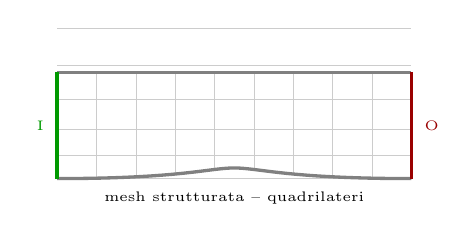
\begin{tikzpicture}[scale=4.5]
    % Visualizzazione schematica della mesh strutturata
    % Nodi verticali con progressione
    \foreach \i in {0,1,...,5} {
      \pgfmathsetmacro{\xL}{0.0}
      \pgfmathsetmacro{\xR}{1.0}
      \pgfmathsetmacro{\y}{\i*0.3/5 + 0.005*\i*\i}
      \draw[gray!40, very thin] (\xL,\y) -- (\xR,\y);
    }
    % Nodi orizzontali con bump
    \foreach \j in {0,1,...,9} {
      \pgfmathsetmacro{\x}{\j/9}
      % calcolo altezza bump
      \pgfmathsetmacro{\bh}{0.03*exp(-25*(\x-0.5)*(\x-0.5))}
      \draw[gray!40, very thin] (\x,\bh) -- (\x,0.3);
    }
    % Parete con bump
    \draw[very thick, gray] (0,0) .. controls (0.35,0) and (0.43,0.03) ..
      (0.5,0.03) .. controls (0.57,0.03) and (0.65,0) .. (1,0);
    % Tetto
    \draw[very thick, gray] (0,0.3) -- (1,0.3);
    % Inlet/Outlet
    \draw[very thick, green!60!black] (0,0) -- (0,0.3);
    \draw[very thick, red!60!black] (1,0) -- (1,0.3);
    % Label
    \node[below, font=\tiny] at (0.5,-0.01) {mesh strutturata -- quadrilateri};
    \node[left, font=\tiny, green!60!black] at (-0.01,0.15) {I};
    \node[right, font=\tiny, red!60!black] at (1.01,0.15) {O};
  \end{tikzpicture}
  \caption{Schema della mesh strutturata per il caso bump (30$\times$60 nodi, quadrilateri).}
  \label{fig:mesh_strutturata_bump}
\end{figure}

\section{Mesh Non Strutturata -- File \texttt{bump\_unstr.geo}}
\label{sec:bump_unstr}

Come secondo approccio si è realizzata una griglia non strutturata con raffinamento
basato su campi attractor/threshold. La geometria è identica al caso strutturato; cambia
solo la strategia di discretizzazione:

\begin{lstlisting}[style=gmsh, caption={File \texttt{bump\_unstr.geo} -- mesh non strutturata con Attractor/Threshold.}, label={lst:bump_unstr}]
// La geometria e' identica a bump.geo (stessi punti, linee, superficie)
// [vedere bump.geo per la definizione della geometria]

// ============================================================
// MESH NON STRUTTURATA con raffinamento adattivo
// ============================================================

// --- Campo attrattore: usa la parete con bump come riferimento ---
Field[1] = Attractor;
// La linea 4 (spline del bump) e' l'attrattore:
// gmsh calcola la distanza di ogni punto del dominio
// dal punto piu' vicino della linea 4
Field[1].EdgeList = {4};

// --- Campo soglia: definisce lc in funzione della distanza ---
Field[2] = Threshold;
Field[2].IField  = 1;        // riferimento al Campo Attractor sopra
Field[2].LcMin   = lc*0.1;   // = 0.005: mesh molto fitta vicino al bump
Field[2].LcMax   = lc*0.5;   // = 0.025: mesh piu' rada lontano dal bump
Field[2].DistMin = h/4;      // = 0.075: distanza sotto cui si usa LcMin
Field[2].DistMax = h/2;      // = 0.150: distanza oltre cui si usa LcMax

// Attivazione del campo
Background Field = 2;

// Conversione in quadrilateri (quando possibile)
Recombine Surface{1};
\end{lstlisting}

\paragraph{Commento sulle scelte del campo Threshold.}
\begin{itemize}
  \item \textbf{\texttt{LcMin = lc*0.1 = 0.005}}: nella zona immediatamente adiacente al bump
    (fino a $d = h/4 = 0.075$ dal profilo), la lunghezza caratteristica è 10 volte più piccola
    di quella di default. Questo garantisce la corretta risoluzione dei gradienti di pressione
    e velocità che si sviluppano vicino alla parete.
  \item \textbf{\texttt{LcMax = lc*0.5 = 0.025}}: nelle zone lontane dal bump, la mesh è 2 volte
    più fine rispetto alla default, un compromesso accettabile per catturare l'evoluzione del
    campo nella regione indisturbata.
  \item \textbf{Transizione}: tra $d = 0.075$ e $d = 0.15$ la lunghezza caratteristica varia
    linearmente, evitando transizioni brusche nella dimensione degli elementi che potrebbero
    degradare la qualità della mesh.
\end{itemize}

\section{Condizioni al Contorno e Parametri della Simulazione}
\label{sec:bump_bc}

I parametri di ingresso al codice CFD sono:

\begin{table}[H]
  \centering
  \caption{Parametri di simulazione -- caso bump.}
  \label{tab:bump_param}
  \begin{tabular}{llll}
    \toprule
    File & Parametro & Valore & Descrizione \\
    \midrule
    \multirow{4}{*}{\texttt{input.txt}}
      & \texttt{KFINAL} & 100\,000 & Numero massimo di iterazioni \\
      & \texttt{KINF}   & 1\,000   & Frequenza di output a schermo \\
      & \texttt{KOUT}   & 1\,000   & Frequenza di salvataggio soluzione \\
      & \texttt{CFL}    & 0.3      & Numero CFL \\
    \midrule
    \multirow{4}{*}{\texttt{inlet.txt}}
      & $T^\circ_{\rm in}$ & 1    & Temperatura totale (adim.) \\
      & $P^\circ_{\rm in}$ & 1    & Pressione totale (adim.) \\
      & $\alpha$           & 0°   & Angolo del flusso in ingresso \\
      & $M_{\rm in}$       & 0.3  & Mach di inizializzazione \\
    \midrule
    \texttt{outlet.txt}
      & $P_{\rm exit}$ & 0.9395 & Pressione statica all'uscita\\
    \bottomrule
  \end{tabular}
\end{table}

Il valore $P_{\rm exit} = 0.9395$ corrisponde alla pressione isentropica per $M = 0.3$:
\begin{equation}
  P_{\rm exit} = \frac{P^\circ}{\left(1 + \dfrac{\gamma-1}{2}M^2\right)^{\gamma/(\gamma-1)}}
  = \frac{1}{\left(1 + 0.2 \times 0.09\right)^{3.5}} \approx 0.9395
\end{equation}

\section{Analisi di Convergenza della Griglia}
\label{sec:bump_convergenza}

\subsection{Raffinamento Progressivo}

L'analisi di convergenza è stata condotta eseguendo simulazioni su quattro griglie progressive,
ciascuna ottenuta raddoppiando approssimativamente il numero di nodi rispetto alla precedente:

\begin{table}[H]
  \centering
  \caption{Griglie utilizzate per l'analisi di convergenza -- bump strutturato.}
  \label{tab:bump_griglie}
  \begin{tabular}{ccccc}
    \toprule
    Caso & $N_{\rm nodi}$ & Nodi orizz.\ & Nodi vert.\ & $\lc$ approx. \\
    \midrule
    1 & 750    & 25  & 30  & 0.022 \\
    2 & 3\,000 & 50  & 60  & 0.011 \\
    3 & 6\,750 & 75  & 90  & 0.007 \\
    4 & 12\,000& 100 & 120 & 0.005 \\
    \bottomrule
  \end{tabular}
\end{table}

\subsection{Campo di Mach e Entropia}

Al raffinamento progressivo della griglia si osservano i seguenti effetti:
\begin{itemize}
  \item Il campo di Mach diventa progressivamente più simmetrico rispetto all'asse verticale
    passante per l'apice del bump, avvicinandosi alla soluzione analitica isentropica.
  \item Il campo di entropia $\bar{S}$, che dovrebbe essere identicamente nullo, presenta valori
    non nulli dovuti alla dissipazione numerica dello schema; tali valori si riducono al
    raffinamento della griglia.
\end{itemize}

\subsection{Norma $L_2$ dell'Entropia e Ordine di Convergenza}

La norma $L_2$ dell'entropia (Eq.~\eqref{eq:norma_entropia}) decresce monotonicamente al
raffinamento. Dalla tabella seguente si ricavano le grandezze dell'analisi di convergenza:

\begin{table}[H]
  \centering
  \caption{Risultati dell'analisi di convergenza -- bump, confronto Lax--Friedrichs vs.\ Roe.}
  \label{tab:bump_convergenza}
  \renewcommand{\arraystretch}{1.25}
  \begin{tabular}{lccccc}
    \toprule
    Metodo & Tipo analisi & $p$ & $u_{\rm esatto}$ & $E$ & GCI \\
    \midrule
    Lax--Friedrichs & Sol.\ esatta nota  & 0.603 & 0       & $1.45\times10^{-3}$ & $4.36\times10^{-3}$ \\
    Roe             & Sol.\ esatta nota  & 0.861 & 0       & $9.11\times10^{-4}$ & $2.73\times10^{-3}$ \\
    \midrule
    Lax--Friedrichs & Ordine teorico     & 1.00  & $9.37\times10^{-4}$ & $5.16\times10^{-4}$ & $1.55\times10^{-3}$ \\
    Roe             & Ordine teorico     & 1.00  & $8.25\times10^{-4}$ & $8.59\times10^{-5}$ & $2.58\times10^{-4}$ \\
    \midrule
    Lax--Friedrichs & Ordine effettivo   & 0.226 & $5.66\times10^{-3}$ & $4.21\times10^{-3}$ & $1.26\times10^{-2}$ \\
    Roe             & Ordine effettivo   & 0.350 & $3.49\times10^{-3}$ & $2.57\times10^{-3}$ & $7.72\times10^{-3}$ \\
    \bottomrule
  \end{tabular}
\end{table}

\paragraph{Interpretazione dei risultati.}
\begin{itemize}
  \item Lo schema di \textbf{Roe} produce errori sistematicamente più piccoli di
    Lax--Friedrichs a parità di griglia, grazie alla minore dissipazione numerica intriseca
    del metodo upwind.
  \item L'ordine di convergenza effettivo ($p \approx 0.6$ per Lax--Friedrichs, $p \approx 0.9$
    per Roe) è inferiore all'ordine teorico di 1 perché le griglie impiegate non sono ancora
    sufficientemente fini da raggiungere la \emph{regione asintotica} in cui i termini di
    ordine superiore nel residuo diventano trascurabili rispetto al termine dominante
    $k h^p$.
  \item I valori di $u_h$ usati nell'analisi sono:
    \begin{align*}
      u_h &= \begin{cases} 1.45\times10^{-3} & \text{Lax--Friedrichs} \\
                           9.11\times10^{-4} & \text{Roe}\end{cases}, &
      u_{2h} &= \begin{cases} 2.17\times10^{-3} & \text{Lax--Friedrichs} \\
                              1.62\times10^{-3} & \text{Roe}\end{cases}, &
      u_{4h} &= \begin{cases} 3.00\times10^{-3} & \text{Lax--Friedrichs} \\
                              2.52\times10^{-3} & \text{Roe}\end{cases}
    \end{align*}
\end{itemize}

\subsection{Considerazioni sulla Scelta dello Schema Numerico}

La superiorità dello schema di Roe in termini di accuratezza è la conseguenza diretta della
sua costruzione: mentre Lax--Friedrichs aggiunge una dissipazione numerica proporzionale a
$\lambda_{\max}(\uvec^R - \uvec^L)$, che non distingue tra onde con velocità diversa,
il solutore di Roe scompone il salto $\uvec^R - \uvec^L$ nelle direzioni proprie della matrice
Jacobiana, applicando la dissipazione corretta per ogni onda caratteristica. Il risultato è
un'interfaccia numerica più netta, con meno smearing delle strutture fisiche. Il costo
computazionale aggiuntivo di Roe è moderato (decomposizione in autovettori a ogni interfaccia)
e ampiamente compensato dall'accuratezza guadagnata.
